%!TEX root = ../masters_thesis.tex

% TODO
% basic idea: given initial state $t_0$, consecutively insert Hivent Operations changing this state
% current state: accumulate all changes
% four domains: semantic, spatial, thematic and temporal
% main difference spatial <-> thematic: no relations between names of two Areas. While it does not make any sense, potentially there could be two Areas active at the same time with exactly the same name. The update of the name of one Area is independent from any other Area. This is not true for the territory: They are highly related to each other. Geospatially each Area has at least one neighbor and two neighbors share the same border. An update of the territory of one Areas results in the update of at least one other territory.
% concrete working of changes: [OldAreas], updateArea, [NewAreas]
% execution of changes (forwards / backwards): hide old areas, show new areas, update updateArea

\section{Hivent Model} % (fold)
\label{sec:hivent_model}

This section proposes the spatio-temporal \emph{Hivent model} to represent countries and their evolution in time and space. In section \ref{sec:spatio_temporal_data_models}, different spatio-temporal data models were introduced. The \emph{Snapshot Model} is unsuitable for the problem space. \emph{Simple Time-Stamping} is helpful to link countries to their history, but it does not explicitly model historical changes, which is desireable. For that purpose, the idea of the \emph{Event-Based Spatio-Temporal Data Model} was developed, but since it only works for raster data, it is also not suitable for this thesis. This problem is solved in the \emph{History Graph Model}. Additionally, the introduced temporal changes allow to represent historical changes and their influences on geographic entities directly in the model. Finally, the \emph{Three-Domain Model} introduces a helpful concept to separate the spatial, temporal and thematic dimension of a spatio-temporal entity.

The Hivent Model is constructed from components of some of these models: It is event-based and supports vector data. It is organized in four domains and allows to visualize data on a graph. The first section \ref{sub:elements} introduces the main elements of the Hivent model. Afterwards, the preconditions are defined in section \ref{sub:preconditions}. One major contribution of this thesis is proposed in section \ref{sub:hivent_operations}: the set of five \emph{Hivent Operations} that describe all possible changes of countries in time and space. This section closes with the \emph{HistoGraph} (section \ref{sub:histograph}), a visualization of the evolution of countries.

% ------------------------------------------------------------------------------
\subsection{Elements} % (fold)
\label{sub:elements}

% - - - - - - - - - - - - - - - - - - - - - - - - - - - - - - - - - - - - - - -
\vspace{-1em}
\paragraph{Hivents} % (fold)
\label{par:hivent}

represent historically significant happenings, e.g. a treaty, bill or declaration.
The word is an acronym for \emph{\textbf{Hi}}storical e\emph{\textbf{vent}}.
The focus in this work is on events that influence the geopolitical situation on Earth.
An Hivent happens at one particular point in time and space and is therefore the main organizing elements of the eponymic data model.

% paragraph hivent (end)

% - - - - - - - - - - - - - - - - - - - - - - - - - - - - - - - - - - - - - - -
\vspace{-1em}
\paragraph{Areas} % (fold)
\label{par:area}

represent one identical current or historical country. They are an abstract entity on the map with a \emph{name} and a \emph{territory}. The name consists of a common \emph{short name}, e.g. ``Germany'' and a \emph{formal name}, e.g. ``Federal Republic of Germany''. The \emph{territory} of the Area is described by a polypolygon, a set of weakly simple polygons to support enclaves and exclaves. The polylines of a polygon consist of an ordered set of points that represent a border of the country. They are either \emph{interior}, i.e. bordering another country, or a \emph{coastline}, bordering a body of water. Additionally, an Area keeps a reference to the historical changes creating, updating and ceasing it.

% paragraph area (end)

% ------------------------------------------------------------------------------
\vspace{-1em}
\paragraph{Historical Changes} % (fold)
\label{par:historical_changes}

influence the evolution of Areas over time. Throughout the lifetime of an Area, it is created at some point $t_s$, then its territory and short name can change multiple times $t_i: t_s < t_i$ and at some point $t_e: t_s < t_i < t_e$ it ceases. Since all changes in this model are sudden, there are only two possible states an Area can be in: It is \emph{active}, if at the current time point it is historically existing and it is \emph{inactive} if it does not. Each Area is \textbf{uniquely identified by its formal name}. That means as soon as the formal name of an Area changes (e.g. ``German Empire'' to ``Federal Republic of Germany''), it is considered a ``new'' Area. Each Historical Change belongs to exactly one Hivent, inheriting its time point at which the change happens.  The change is described by a Hivent Operation introduced in section \ref{sub:hivent_operations}.

\begin{figure}[H]
  \vspace{1em}
  \centering
  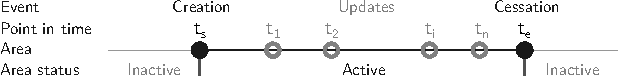
\includegraphics[width=0.9\textwidth]{graphics/development/hivent_model/area_states}
  \caption{Three event types that change Areas, resulting in two different area states}
  \label{fig:area_states}
\end{figure}


% paragraph historical_changes (end)

% subsection section area (end)

% ------------------------------------------------------------------------------
\subsection{Preconditions} % (fold)
\label{sub:preconditions}

\begin{quoteit}
In the beginning God created the heavens and the Earth \\
Now the Earth was formless and empty [...] \\
And God said, “Let there be light” --- and there was light.
\end{quoteit}
\vspace{-1em}
\hfill -- Genesis 1:1, The First Book of Moses, Old Testament

There are five axoims and two assumptions the Hivent Model is based on. The theoretical foundation is the model of the Earth and its curved surface that can be projected on a two-dimensional map using a map projection, as introduced in sections \ref{sub:model_of_geographical_space}.

\vspace{-1.0em}
\newtheorem{invariant_surface}[assicounter]{Axiom}
\begin{invariant_surface}
\label{axm:invariant_surface}
  The Earth's surface has an invariant area size, i.e. it does not change over time.
\end{invariant_surface}

\vspace{-2.5em}
\newtheorem{area_on_surface}[assicounter]{Axiom}
\begin{area_on_surface}
\label{axm:area_on_surface}
  Each Area in the spatio-temporal system is located directly on the surface of the Earth.
\end{area_on_surface}

These axiom sets the spatial foundation of the system: a constant dimension of the map and Areas covering the map. The basis of the temporal part of the system is content of the next three axioms:

\vspace{-1.0em}
\newtheorem{initial_configuration}[assicounter]{Axiom}
\begin{initial_configuration}
\label{axm:initial_configuration}
  The spatio-temporal system has an initial state at time point $t_0$. At this initial state, there exists exactly one Area, denoted by $\Omega$ and referred to as the \emph{universe} Area. It has no name and its territory covers the whole surface of the Earth.
\end{initial_configuration}

\vspace{-2.5em}
\newtheorem{historical_change}[assicounter]{Axiom}
\begin{historical_change}
\label{axm:historical_change}
  At each time point $t_i \geq t_0$ multiple historical changes can be introduced.
\end{historical_change}

\vspace{-2.5em}
\newtheorem{unique_coverage}[assicounter]{Axiom}
\begin{unique_coverage}
\label{axm:unique_coverage}
  At each time point $t_i \geq t_0$ each point on the surface of the Earth is covered by exactly one territory of exactly one Area.
\end{unique_coverage}

As it has been defined in section \ref{par:historical_changes}, an Historical Change can create, manipulate and cease Areas on the Earth's surface. According to axoim \ref{axm:unique_coverage}, each change introduced in the system must maintain the spatial integrity on the map: When an Area with a territory is created on the map, the Area claiming this territory before has to cease it. Formally, it can be said that each change consists of a set of old Areas $A$ that are manipulated, a set of new Areas $B$ that are created in the change, and an operation $\rightarrow_C$ describing the change. Each Area $A_i \in A$ and $B_i \in B$ has a territory $A_i^T$  respectively $B_i^T$. For each change introduced in the system, the territories of the old Areas must have the same size than the territories of the new Areas to maintain the spatial integrity of axiom \ref{axm:unique_coverage}:
\begin{align*}
  \bigcup\limits_{i=1}^n A_i^T ~\textbf{=}~ \bigcup\limits_{i=1}^n B_i^T
\end{align*}

The first changes introduced in the system at time point $t_0$ are the creation of all bodies of water, including the oceans and lakes, denoted as $W$. Each Area $W_i \in W$ is created with their name and territory cut out of $\Omega$. The result is that after $t_0$, the map is divided into water ($W$) and land ($\Omega$). Land can at any point in time be either \emph{claimed}, i.e. it is currently occupied by the territory of exactly one active Area, or on a contrary be \emph{unclaimed}, i.e. belonging to $\Omega$. It is a subtractive data model, because each new Areas territory is cut out of $\Omega$.

\begin{figure}[H]
  \centering
  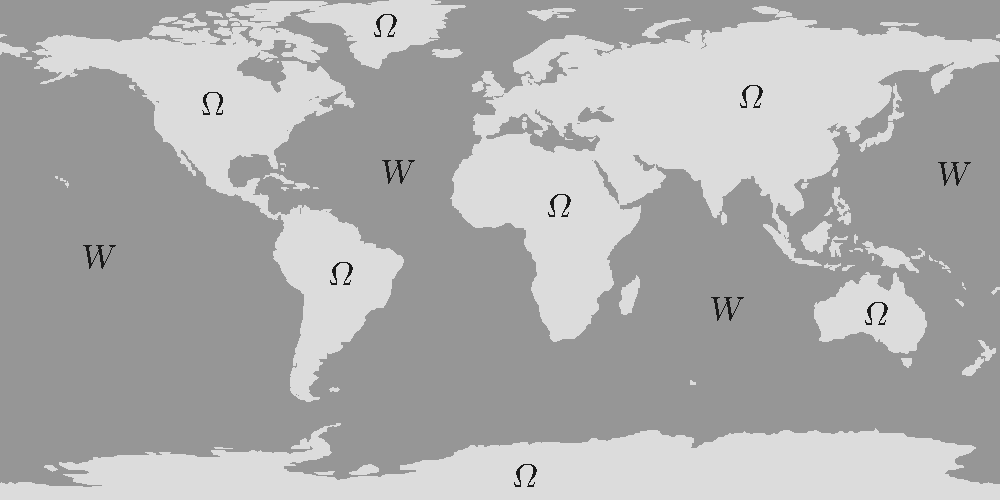
\includegraphics[width=0.5\textwidth]{graphics/development/hivent_model/init_map}
  \caption{The initial state of the world map at time point $t_0$}
  \label{fig:init_map}
\end{figure}

In the real world, the name of a country changes according to sudden events, e.g. a declaration or a governmental bill. The territory can change either because of a geographical processes, e.g. the sea level rise influencing the change of the coastline, or according to a historical event, e.g. a treaty. The Hivent model is based on two assumptions that simplify the model and keep the problem space clear:

\vspace{-1.0em}
\newtheorem{coastline_territory}[assicounter]{Assumption}
\begin{coastline_territory}
\label{axm:coastline_territory}
  The territory of a country stops at the coastline.
\end{coastline_territory}

\vspace{-2.0em}
\newtheorem{constant_coastlines}[assicounter]{Assumption}
\begin{constant_coastlines}
\label{axm:constant_coastlines}
  The spatial configuration of water and the coastlines have not changed over time.
\end{constant_coastlines}

Both assumptions are obviously wrong: In line with \cite{UNSeaBorders}, the territory of a country extends in a range of 3 to 12 miles (5 to 20 kilometers) into international waters. They are constantly changing and so does the distribution of land and water on Earth. However, the assumptions allow the Hivent Model to focus only on discrete historical changes. It is subject to future work to extend the data model to account for long-term processes that change water and the coastlines. For now, the temporal behavior of an Area in the Hivent Model can be described as a \emph{static object that changes according to sudden events}.

% base: Newtons concept of absolute space?
% TODO: topological rule?
% each border has exactly two neighboring Areas
% each Area has at least one neighboring Area

% subsection preconditions (end)

% ------------------------------------------------------------------------------
\subsection{Hivent Operations} % (fold)
\label{sub:hivent_operations}

Respecting the preconditions, there are several different types of changes that transform a set of old Areas $A$ to a set of new Areas $B$. All possible changes can be expressed with only five spatio-temporal operations that are called \emph{Hivent Operations}. The first four change the identity of a set of Areas and therefore establish historical predecessor-successor-relationships. They are always symmetric, i.e. if one old Area is replaced by one new Area, the old Area is the historical predecessor of the new Area and vice versa the new Area is the successor of the old Area. The last operation changes an aspatial property of an Area.

\begin{description}

  \item[UNI -- Unification]
  A set of old Areas unifies to one new Area. The old Areas cease, becoming the historical predecessors of the new Area. The territory of this new Area is the union of the territories of the old Areas. The new Area receives a new name. \\[0.25em]
  \begin{footnotesize}
    In 1922, the Russian SFSR, the Transcaucasian SFSR, the Ukrainian SSR and the Byelorussian SSR unified and formed the Union of Soviet Socialist Republics (USSR).
  \end{footnotesize}

  \item[INC -- Incorporation]
  One or more old Areas are incorporated into another Area that stays active. Its territory is enlarged by the union of the territories of the old Areas. The old Areas are historical predecessors of the Area that stays active. \\[0.25em]
  \begin{footnotesize}
    In 1990, the territory of the German Democratic Republic (East Germany) became part of the Federal Republic of Germany (West Germany). Although this event is known as the \emph{German Reunification}, it is historically an incorporation of East Germany into West Germany \cite{incorporationEastWestGermany}.
  \end{footnotesize}

  \item[SEP -- Separation]
  As the inverse of unification, one old Area is separated into multiple new Areas. Each new Area gets a part of the territory of the old Area, receives a new name, and has the old Area as its only historical predecessor. \\[0.25em]
  \begin{footnotesize}
    In 1993, the Czech and Slovak Federal Republic, commonly known as Czechoslovakia, dissolved into present-day Czech Republic and Solvak Republic, creating two new countries out of one old.
  \end{footnotesize}

  \item[SEC -- Secession]
  As the inverse of incorporation, one or more new Areas are ceded from a previously existing Area that stays active. Each new Area gets a new name, receives the previously existing Area as the only historical predecessor and a part of its territory. \\[0.25em]
  \begin{footnotesize}
    In 2008, the Republic of Kosovo declared independence from Serbia and has since then partially received international recognition. Serbia stays a country, keeping its name, but ceding a part of its territory to Kosovo.
  \end{footnotesize}

  \item[NCH -- Name Change]
  An Area changes its short name but preserves its formal name and identity. \\[0.25em]
  \begin{footnotesize}
    A recent change happened on 5. May 2016: The cabinet of Czech Republic approved that the country will now offically be called ``Czechia''. However, the formal name stays ``Czech Republic'', which preserves its identity.
  \end{footnotesize}
\end{description}

\vspace{1.5em}
\begin{table}[H]
\begin{center}
\begin{tabular}{cx{2.5cm} cx{2.5cm} cx{2.5cm} cx{2.5cm} cx{2.5cm}}

  \toprule
  \texttt{UNI} & \texttt{INC} & \texttt{SEP} & \texttt{SEC} & \texttt{NCH} \\
  Unification & Incorporation & Separation & Secession & Name Change \\[1em]

  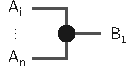
\includegraphics{graphics/development/hivent_model/operations/UNI} &
  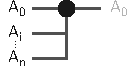
\includegraphics{graphics/development/hivent_model/operations/INC} &
  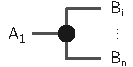
\includegraphics{graphics/development/hivent_model/operations/SEP} &
  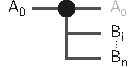
\includegraphics{graphics/development/hivent_model/operations/SEC} &
  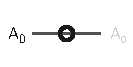
\includegraphics{graphics/development/hivent_model/operations/NCH} \\

  \bottomrule
\end{tabular}
\caption{The five Hivent Operations}
\label{tab:hivent_operations}
\end{center}
\end{table}

% subsection hivent_operations (end)

% ------------------------------------------------------------------------------
\subsection{HistoGraph} % (fold)
\label{sub:histograph}

Based on the idea of the History Graph Model (section \ref{fig:history_graph_model}), the linguistically and conceptually related \emph{HistoGraph} visualizes the evolution of countries in time, without any spatial relation. The edges of the graph represent an Area, the nodes a Hivent Operation. The graph shows the predecessor-successor-relationships between Areas. This is easily possible, because in the Hivent Model an Area keeps references to the historical changes creating, updating and ceasing the Area (section \ref{par:area}).

The two-dimensional HistoGraph has an horizontal orientation. The x-axis refers to one time point, the y-axis has no spatio-temporal relation and depends how much space it needs. The graph uses the visualization approach of the five Hivent Operations (table \ref{tab:hivent_operations}), including the following symbols:

\begin{table}[H]
\begin{center}
\begin{tabular}{c l l}

  \raisebox{3.5\height}
  {
\includegraphics{graphics/development/hivent_model/histograph/line}}
  & Area
  & \\

  \raisebox{-0.2\height}
  {
\includegraphics{graphics/development/hivent_model/histograph/circle_filled}}
  & Identity-changing Hivent Operation
  & \texttt{UNI}, \texttt{INC}, \texttt{SEP}, \texttt{SEC} \\

  \raisebox{-0.2\height}
  {
\includegraphics{graphics/development/hivent_model/histograph/circle_unfilled}}
  & Property-changing Hivent Operation
  & \texttt{NCH} \\

  \raisebox{-0.2\height}
  {
\includegraphics{graphics/development/hivent_model/histograph/circle_combo}}
  & A combination of both
  & e.g. \texttt{INC + NCH}

\end{tabular}
\label{tab:histograph_symbols}
\end{center}
\end{table}

\vspace{-2em}

Each uninterrupted horizontal line refers to exactly one Area. If an horizontal line leads straight through a circle, the identity of the Area is preserved in the operation. New Areas resulting from an identity-changing Hivent Operation emerge from the circle with a vertical line, indicating a sudden change with zero duration. From this line, the new Areas branch out right-angled. The HistoGraph is created from one particular reference Area. It visualizes historically related Areas in one direction: into the past, it recursively plots the predecessors on the graph, but not the predecessors successors. Into the future, the successors of the reference Area are plotted recursively, but not their predecessors.

The behavior of the HistoGraph is shown in figure \ref{fig:example_germany} at the example of present-day Germany and its state history since the end of World War II. This history is driven by six historical events, which provide examples for all five Hivent Operations. They are listed in table \ref{tab:german_history_since_1945}.

\begin{figure}[ht]
  \vspace{0.5em}
  \centering
  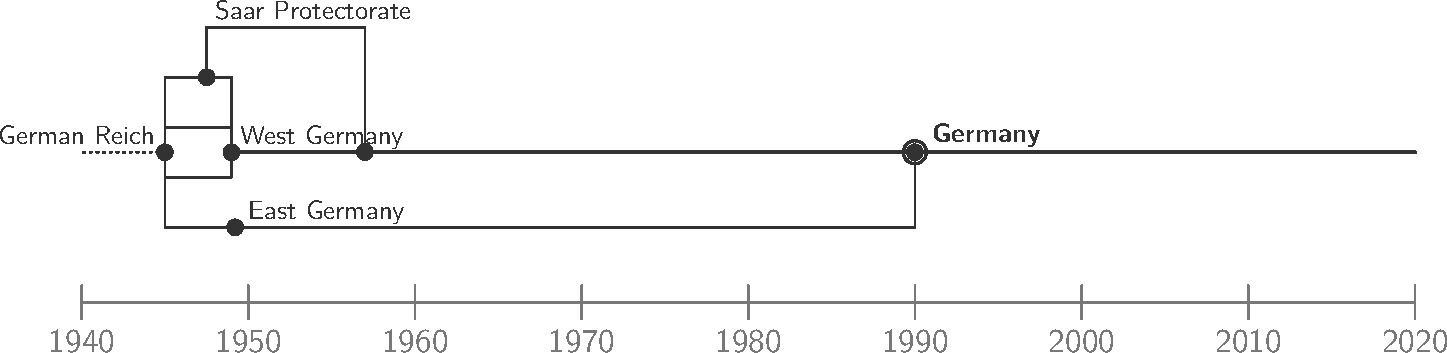
\includegraphics[width=0.8\textwidth]{graphics/development/hivent_model/histograph/example_germany}
  \caption{The concept of the HistoGraph at the example of the history of Germany since 1945}
  \label{fig:example_germany}
\end{figure}


\begin{table}[ht]
\begin{center}
\begin{tabular}{l p{8.5cm} l}
  \toprule
  Hivent date & Hivent description & Hivent Operations \\
  \midrule

    05.06.1945
  & \footnotesize{In the Berlin Declaration the total dissolution of the Third Reich is confirmed. It separates into multiple parts, returning the territories annexed by the German Reich in World War II. The rest is controlled by the British, French, American and Soviet occupation zone.}
  & \texttt{SEP} \\

    16.02.1946
  & \footnotesize{The Saar Protectorate is entangled from the French Zone of Occupation Germany, creating an own country.}
  & \texttt{SEC} \\

    28.05.1949
  & \footnotesize{The Federal Republic of Germany (West Germany) is created from the British, American and French Zone of Occupation.}
  & \texttt{UNI} \\

    07.10.1949
  & \footnotesize{The German Democratic Republic (East Germany) is created from the Soviet Zone of Occupation.}
  & \texttt{UNI} \\

    01.01.1957
  & \footnotesize{The Saar Treaty (``Little Reunification'') joins the Saar Protectorate as the Bundesland Saarland in West Germany.}
  & \texttt{INC} \\

    03.10.1990
  & \footnotesize{In the German Reunification, East Germany joins West Germany. The Federal Republic of Germany is now just called ``Germany''.}
  & \texttt{INC + NCH} \\

  \bottomrule
\end{tabular}
\caption{Historical events in German state history since 1945}
\label{tab:german_history_since_1945}
\end{center}
\end{table}

The example hosts a special case: in October 1949, East Germany was created from the Soviet Zone of Occupation. Both Areas have the same territory, but a different short and formal name. A \texttt{NCH} can not be performed, because the identity is not preserved: The German Democratic Republic is a new Area. However, the change can be described by a \texttt{UNI} of only one Area (Soviet zone), creating a new Area (East Germany) and establishing a historical relationship between both.

The graph plots Germany first. Since it does not have any successors, the plot goes only one way, historically backwards: East Germany and the Saar Protectorate were incorporated into Germany, so they are plotted. They emerged from the four post-war occupation zones, visualized next. All of the four occupation zones themselves originated from the German Reich. However, the Reich dissolved into many more Areas, e.g. the Memel territory. They are not included in the graph, because they are not predecessors of any Area that is a recursive predecessor of present-day Germany.

Many problems of the graph visualization are apparent in this example: Circles my overlap, if many operations happen in a short period of time -- in this case between 1945 and 1949.
The name ``West Germany'' collides with the vertical line indicating the incorporation of the Saar Protectorate, which should also be avoided.
Additionally, the names of the Areas of the four post-war occupation zones can not be shown in the graph, because there is no space for them.
One more important aspect can be seen in the creation of West Germany in 1949: A \texttt{UNI} operation unifies three old Areas to one new Area. This could be visualized symmetrically with a straight line from the midmost incoming Area line into the circle to the outgoing Area line of the new Area. This would give the wrong impression that this midmost Area has the same identity than the newly created Area. In general, the circle for \texttt{UNI} and \texttt{SEP} operations with an odd number of old respectively new Areas must be displaced off the center to emphasize that the identity has changed.
All these issues are not in the scope of this thesis and subject to future work in the field of Information Visualization.

% subsection histograph (end)

% section hivent_model (end)